% Options for packages loaded elsewhere
\PassOptionsToPackage{unicode}{hyperref}
\PassOptionsToPackage{hyphens}{url}
%
\documentclass[
]{article}

% Use endnotes rather than footnotes.
\usepackage{endnotes}
\let\footnote=\endnote

% Double-space the bibliography
\usepackage{setspace}

\title{How Scholars Quote from Source Texts: a Case for Corpus-Adapted
Text-Reuse Detection}
\author{Jonathan Reeve \and Sierra Eckert \and Milan Terlunen}
\date{}

\usepackage{amsmath,amssymb}
\usepackage{lmodern}
\usepackage{iftex}
\ifPDFTeX
  \usepackage[T1]{fontenc}
  \usepackage[utf8]{inputenc}
  \usepackage{textcomp} % provide euro and other symbols
\else % if luatex or xetex
  \usepackage{unicode-math}
  \defaultfontfeatures{Scale=MatchLowercase}
  \defaultfontfeatures[\rmfamily]{Ligatures=TeX,Scale=1}
\fi
% Use upquote if available, for straight quotes in verbatim environments
\IfFileExists{upquote.sty}{\usepackage{upquote}}{}
\IfFileExists{microtype.sty}{% use microtype if available
  \usepackage[]{microtype}
  \UseMicrotypeSet[protrusion]{basicmath} % disable protrusion for tt fonts
}{}
\makeatletter
\@ifundefined{KOMAClassName}{% if non-KOMA class
  \IfFileExists{parskip.sty}{%
    \usepackage[skip=0pt, indent=40pt]{parskip}
  }{% else
    \setlength{\parindent}{0pt}
    \setlength{\parskip}{6pt plus 2pt minus 1pt}}
}{% if KOMA class
  \KOMAoptions{parskip=half}}
\makeatother
\usepackage{xcolor}
\IfFileExists{xurl.sty}{\usepackage{xurl}}{} % add URL line breaks if available
\IfFileExists{bookmark.sty}{\usepackage{bookmark}}{\usepackage{hyperref}}
\hypersetup{
  pdftitle={How Scholars Quote from Source Texts: a Case for Corpus-Adapted Text-Reuse Detection},
  pdfauthor={Jonathan Reeve; Sierra Eckert; Milan Terlunen},
  hidelinks,
  pdfcreator={LaTeX via pandoc}}
\urlstyle{same} % disable monospaced font for URLs
\usepackage{longtable,booktabs,array}
\usepackage{calc} % for calculating minipage widths
% Correct order of tables after \paragraph or \subparagraph
\usepackage{etoolbox}
\makeatletter
\patchcmd\longtable{\par}{\if@noskipsec\mbox{}\fi\par}{}{}
\makeatother
% Allow footnotes in longtable head/foot
\IfFileExists{footnotehyper.sty}{\usepackage{footnotehyper}}{\usepackage{footnote}}
\makesavenoteenv{longtable}
\usepackage{graphicx}
\makeatletter
\def\maxwidth{\ifdim\Gin@nat@width>\linewidth\linewidth\else\Gin@nat@width\fi}
\def\maxheight{\ifdim\Gin@nat@height>\textheight\textheight\else\Gin@nat@height\fi}
\makeatother
% Scale images if necessary, so that they will not overflow the page
% margins by default, and it is still possible to overwrite the defaults
% using explicit options in \includegraphics[width, height, ...]{}
\setkeys{Gin}{width=\maxwidth,height=\maxheight,keepaspectratio}
% Set default figure placement to htbp
\makeatletter
\def\fps@figure{htbp}
\makeatother
\setlength{\emergencystretch}{3em} % prevent overfull lines
\providecommand{\tightlist}{%
  \setlength{\itemsep}{0pt}\setlength{\parskip}{0pt}}
\setcounter{secnumdepth}{-\maxdimen} % remove section numbering
\newlength{\cslhangindent}
\setlength{\cslhangindent}{1.5em}
\newlength{\csllabelwidth}
\setlength{\csllabelwidth}{3em}
\newlength{\cslentryspacingunit} % times entry-spacing
\setlength{\cslentryspacingunit}{\parskip}
\newenvironment{CSLReferences}[2] % #1 hanging-ident, #2 entry spacing
 {% don't indent paragraphs
  \setlength{\parindent}{0pt}
  % turn on hanging indent if param 1 is 1
  \ifodd #1
  \let\oldpar\par
  \def\par{\hangindent=\cslhangindent\oldpar}
  \fi
  % set entry spacing
  \setlength{\parskip}{#2\cslentryspacingunit}
 }%
 {}
\usepackage{calc}
\newcommand{\CSLBlock}[1]{#1\hfill\break}
\newcommand{\CSLLeftMargin}[1]{\parbox[t]{\csllabelwidth}{#1}}
\newcommand{\CSLRightInline}[1]{\parbox[t]{\linewidth - \csllabelwidth}{#1}\break}
\newcommand{\CSLIndent}[1]{\hspace{\cslhangindent}#1}
\makeatletter
\@ifpackageloaded{subfig}{}{\usepackage{subfig}}
\@ifpackageloaded{caption}{}{\usepackage{caption}}
\captionsetup[subfloat]{margin=0.5em}
\AtBeginDocument{%
\renewcommand*\figurename{Fig.}
\renewcommand*\tablename{Table}
}
\AtBeginDocument{%
\renewcommand*\listfigurename{List of Figures}
\renewcommand*\listtablename{List of Tables}
}
\newcounter{pandoccrossref@subfigures@footnote@counter}
\newenvironment{pandoccrossrefsubfigures}{%
\setcounter{pandoccrossref@subfigures@footnote@counter}{0}
\begin{figure}\centering%
\gdef\global@pandoccrossref@subfigures@footnotes{}%
\DeclareRobustCommand{\footnote}[1]{\footnotemark%
\stepcounter{pandoccrossref@subfigures@footnote@counter}%
\ifx\global@pandoccrossref@subfigures@footnotes\empty%
\gdef\global@pandoccrossref@subfigures@footnotes{{##1}}%
\else%
\g@addto@macro\global@pandoccrossref@subfigures@footnotes{, {##1}}%
\fi}}%
{\end{figure}%
\addtocounter{footnote}{-\value{pandoccrossref@subfigures@footnote@counter}}
\@for\f:=\global@pandoccrossref@subfigures@footnotes\do{\stepcounter{footnote}\footnotetext{\f}}%
\gdef\global@pandoccrossref@subfigures@footnotes{}}
\@ifpackageloaded{float}{}{\usepackage{float}}
\floatstyle{ruled}
\@ifundefined{c@chapter}{\newfloat{codelisting}{h}{lop}}{\newfloat{codelisting}{h}{lop}[chapter]}
\floatname{codelisting}{Listing}
\newcommand*\listoflistings{\listof{codelisting}{List of Listings}}
\makeatother
\ifLuaTeX
  \usepackage{selnolig}  % disable illegal ligatures
\fi

\begin{document}
\maketitle

\doublespacing

\hypertarget{abstract}{%
\section{Abstract}\label{abstract}}

Using text-reuse detection, we develop a tool for analyzing quotations
from source texts in a body of scholarly writing. While text-reuse
detection algorithms in general have been increasingly used within
computational literary studies and adjacent computational fields, less
attention has been paid to the specific challenges of using these
algorithms to detect quotations from source texts. We use our tool to
analyze quotations from a source text (George Eliot's
\emph{Middlemarch}) within a collection of JSTOR-held scholarly writing
in order to demonstrate the need for corpus-adapted text-reuse
detection. By this we mean methods of text-reuse detection tuned to the
text structures of specific corpora. Our methodology traces not only how
and where a text has been quoted, but also enables a more granular
analysis of what parts have been quoted and how this has developed over
time. Bringing text-reuse detection together with rich bibliographic
metadata, we showcase the strengths of this local, more corpus-specific
method for identifying quotations.

\hypertarget{introduction}{%
\section{Introduction}\label{introduction}}

Quotations, acts of plagiarism, instances of repeating gene
sequences---these represent just a small fraction of the different kinds
of objects that a researcher might be after when they look for instances
of text reuse. Within the context of computational scholarship,
text-reuse detection-----or the algorithmic identification of strings
that appear in two sets of text-----has benefited from its ecumenical
approach to texts. The ability to trace the reappearance of a portion of
one text in another text is useful for understanding many humanistic
domains that cite and use sources, from law to historiography, as well
as in scientific realms such as genomics that deal with repetitive data
sequences such as DNA. Such methods offer a wide range of disciplines
the ability to trace instances of textual borrowing, replication or
reuse.

Despite being applicable to a very broad range of objects, text-reuse
detection as a method has often been deployed to answer a narrower
research question: \emph{is} there a possibility that portions of one
text or corpus appear in another? Often the aim is to determine the
possibility of plagiarism or textual borrowing. However, this
assumption, and the assumption that identical methods can be used
equally well for any text or corpus, have limited researchers' ability
to effectively study text reuse for purposes other than detecting
\emph{covert} borrowing or plagiarism. Quotation, and quotation in
scholarly writings in particular, is a kind of text reuse that is not
secretive or concealed, and has distinctive conventions for signaling
and demarcating reused portions of text, as well as norms around what
properly counts as quotation in contrast to paraphrase (or plagiarism).
Text-reuse detection methods developed to identify everything from
genetic similarities to plagiarized computer code will have only limited
success in detecting the distinctive text-reuse practice that forms the
bedrock of much scholarly writing.

Quotation is particularly central to literary scholarship, where
well-established disciplinary practices of close reading and textual
exegesis give quotations from source texts a particular role in literary
scholars' argumentation. As such, instead of asking \emph{if} there's a
possibility that one text includes portions of another (as in plagiarism
detection), our study of scholarly quotation presupposes that most texts
\emph{do} quote from their sources. Based on this expectation, we
develop a text-reuse detection tool adaptable to the given corpora. This
tool offers fuzzy matching and hyperparameters that respond to typical
features of coropora of scholarly writing, which a researcher can
fine-tune to the specificities of their corpus and research question.
While our case study is literary scholarship, the methods we outline for
corpus-adapted text-reuse detection could apply (no doubt with
modifications) to the conventions around quotation of sources in other
disciplines across the humanities and social sciences. Our central
argument is that using text-reuse detection to study scholarly
quotations can be improved through methods that take into account norms
and conventions of scholarly writing, and in turn will allow scholars to
ask more nuanced questions relevant to their discipline and objects of
study. Our preliminary findings, which analyze matches between George
Eliot's \emph{Middlemarch} and thousands of scholarly writings from
JSTOR, show the benefits of corpus-adapted methods in linking
computational text analysis with disciplinary history.\footnote{For the
  code, relevant data, and further analysis related to our text matcher,
  please see our GitHub repository:
  https://github.com/lit-mod-viz/middlemarch-critical-histories}

\hypertarget{background}{%
\section{Background}\label{background}}

Computational text-reuse detection has benefited from development in
several specific domains. Plagiarism detection, a special use-case of
text-reuse detection, was primarily developed to solve, as one 1981 work
puts it, `the problem of plagiarism in programming assignments by
students in computer science courses' (Donaldson et al., 1981). A
computer science programming assignment, however, differs greatly from
published scholarly writing. For one, whitespace and punctuation are
significant. In addition, plagiarism detection typically looks either at
whole-document similarity or locally replicated syntax (since variables
can be renamed in code, or words can be replaced in a paper using a
thesaurus). There have been several useful overviews of the state of the
plagiarism detection problem, a long-standing problem in natural
language processing (Lukashenko et al., 2007). As plagiarism detection
has grown into a multi-billion dollar industry, it has also become a
lucrative commercial product as private companies have carried forward
and developed its methods outside of the realm of scholarly or
open-source research. (McMurtrie, 2019)\footnote{Both the ethics of
  plagiarism detection and the ethics of proprietary plagiarism
  software---such as Turnitin---have already received critiques for both
  the simplistic understanding of plagiarism and its murky retention of
  student and instructor intellectual property.}

Text-reuse detection has also been used in genomics and bioinformatics
generally. The task of gene sequencing has led to the use of sequence
alignment algorithms, which have undergone various developments over the
years (Li and Homer, 2010). Given two strings of genetic sequences
comprising cytosine {[}C{]}, guanine {[}G{]}, adenine {[}A{]} and/or
thymine {[}T{]}, the algorithm aligns them, such that the common parts
of the sequence have identical indices.

One of the most well-known gene sequence alignment algorithms is BLAST
(Basic Local Alignment Search Tool) from 1990 (Altschul et al., 1990).
As with plagiarism detection, this problem differs greatly from that of
scholarly quotation, in that the possible elements are completely
consistent and few in number (A\textbar C\textbar G\textbar T). With
quotation from literary sources, the elements to be sequenced
potentially include every word in a language. Moreover, verb and noun
forms may be changed in order to fit the scholar's syntax (`he was
``descend{[}ing{]} down the staircase''\,'), variant spellings may
appear (because of British vs American English, because of historical vs
modernized spellings) and, since human memory is involved, even
misquotations sometimes make it into print.

In the early 2000s, methods for studying text-reuse began to make their
way from plagiarism detection and bio-informatics into computational
linguistics. Some of the early methods were oriented around tracking the
reuse of newswire stories from the AP or Reuters in other newspapers
(Clough et al., 2002; Seo and Croft, 2008; Bär et al., 2012) or the
study of plagiarism communities (Khritankov et al., 2015), while others
developed methods for detecting repeated sequences of text incidentally,
as part of generating hyperlinks between different parts of the Google
Books corpus (Kolak and Schilit, 2008).

Text-reuse detection has, more recently, been used by scholars to
identify communities produced by the reprinting of texts, particularly
in newspapers and periodicals. In their work on the Viral Texts Project,
Ryan Cordell, David Smith, and Elizabeth Maddock Dillon have shown how
reprinted poems, ads, and short news articles in 18th-and 19th-century
American newsprint can illuminate patterns in newspaper syndication
(Smith et al., 2013; Smith et al., 2014). Their work has paved the way
for other scholarship on reprinting, including newspapers in other
languages, (Vesanto, Nivala, et al., 2017; and Vesanto, Ginter, et al.,
2017 both apply the BLAST algorithm to Finnish newspapers in the
18th-19th century) and towards different aims, like tracing the
recirculation networks of newswire copy in the corpora of 21st-century
news articles from the US and the UK (Nicholls, 2019). In a similar vein
as text-reuse in literary studies, computational linguistics have used
similar methods in examining how the text of a given policy document is
reprinted in other bills and legislative texts (Linder et al., 2020).
Here, while occasional attention is paid to the particular texts that
`go viral,' the focus is not on particular passages but on the networks
of publishers, syndicators, and editors that such acts of reprinting
reveal.

Early examples of literary scholarship that used text-reuse detection
were modeled after these gene-sequencing and plagiarism detection
methods and, as a consequence, text-reuse methods were shaped around a
particular problem: identifying any instances of potential similarity
between two collections of texts.\footnote{We might contrast the
  assumptions of text-reuse detection with textual versioning and
  collation methods, like the GNU program \texttt{diff}. While
  \texttt{diff} assumes that texts will be near identical: they will
  share text and word or with a few small variations, text-reuse
  detection presumes that two texts will be mostly different, with very
  few shared n-grams.} Scholars were chiefly interested in the potential
evidence of literary borrowing, using BLAST algorithms to find evidence
that eighteenth-century reference texts borrowed passages from Diderot's
and D'Alembert's encyclopedias, (Olsen et al., 2011) or whether
19th-century French writers like Balzac and Gautier plagiarized from one
another (Ganascia et al., 2014).

When computational studies have focused on quotation, they have
typically focused on quotation of passages from canonical source texts
(often, texts from Greek and Roman antiquity or the Hebrew or Christian
Bible) in other non-scholarly texts such as newspapers or novels (Geßner
et al., 2013). Lincoln Mullen, in America's Public Bible, focuses on
quotations from the Old and New Testaments of the Bible in a corpus of
American 18th- and 19th-century newspapers (Mullen, 2016, 2022). Marco
Büchler's TRACER project offers something of a hybrid between the study
of particular quotations and their circulation: TRACER focuses on
reprinting of Classical Greek authors within a corpus of Greek
historian's reference texts and takes frequent quotation as a metric for
a work's `influence.' (Büchler et al., 2013; Kokkinakis and Malm, 2016;
see also Frederik Arnold's {``Lotte''} (later renamed {``Quid''})
framework Arnold, 2022a, 2022b; Arnold and Jäschke, n.d.). Detecting
quotations within texts poses particular challenges: what edition and
translation of the Bible to use, or how to deal with slight
misquotations (Duhaime, 2016; Roe et al., 2016). Recent work has also
begun to extend text-reuse methods to non-Latin scripts (Sturgeon, 2018;
Budak et al., 2021; Budak and Rominger, 2022).

A related but distinct area of scholarship to the study of text reuse is
the study of \emph{citations}, which often goes by the name
`bibliometrics.' Whereas quotation involves the verbatim replication of
some portion of the source text, citation involves only a reference. In
the case of scholarly writings, this is usually a bibliographical
reference formatted according to a citation style determined by the
publisher. For example, to \emph{cite} Michel Foucault's concept of the
`author-function' or the article `What is An Author?' from which it
derives is distinct from quoting his specific formulations within the
article. Citations have particular significance for scholars within the
contemporary university, where they are a widely-used metric that shape
career opportunities. Many decades of research have demonstrated that
the distribution of citations in academia replicates and reinforces
broader inequalities related to social categories like gender and race
(see e.g. Ferber, 1986; Earhart et al., 2021; Smith, 2017). Focused as
they are on the social status of the cited works' authors, these studies
don't typically examine the smaller scale of which portions of a work
are cited (see Romanello, 2016 for an exception, which also analyzes the
book and line numbers included in citations of classical texts like
Vergil's \emph{Georgics}). Methodologically, all these studies function
not by detecting text reuse but by tallying bibliographical references,
which in scholarly writing have a relatively consistent form
(e.g.~in-line citations; footnotes; endnotes; list of works cited). In
contrast, our method detects instances of text reuse, whether
accompanied by a bibliographical reference or not, and doesn't detect
bare citations without quotation. While bare citation is the norm in
certain natural sciences, across the humanities and in literary studies
in particular, quoting from and citing a source are both options, whose
dynamics we want to understand better. It may be, for example, that whom
scholars choose to quote, as opposed to merely cite, further intensifies
the social inequalities already well-documented in citation
patterns.\footnote{Literary scholars have also studied quotation
  practices using various non-digital methods. Studies focusing on the
  presence of quotations in literary works include Meyer (2015);
  Compagnon (1979); Prins (1999); Buurma (2012); and Hack (2016).
  Studies of how portions of literary texts have circulated in the form
  of quotations include Garber (1999); Price (2000); Dames (2010); and
  Mole (2017). Closest to our own project, there have been several
  recent (non-computational) studies examining how \emph{literary
  scholars} quote: Auyoung (2020) and Kramnick (2020).}

Our text-matcher builds on these existing bodies of work by developing
methods geared towards a more specific research task: detecting
quotations from source texts used in scholarly writing. Text-reuse
detection in the contexts of plagiarism or networks of reprinting cast a
wide net (i.e.~set the threshold for detecting reuse lower) in order to
capture as many potential instances as possible, which can then be
further investigated manually as needed. In contrast, our methodology
sets the threshold higher, since scholarly norms presuppose precise
replication in quoted texts, with only limited variants permissible. In
focusing on the quotation of source texts within scholarship, we build a
tool with the aim of identifying quotations in corpora (scholarly
writings) that have more standard conventions for direct quotation. In
doing so, we take inspiration from several recent digital projects
studying scholarly quotation patterns in aggregate. JSTOR Labs and Derek
Miller have analyzed quotations from literary texts in scholarly
writings: both projects present interactive web visualizations for
exploring what lines have been most quoted within Shakespeare's corpus
(Humphreys, 2017; Miller, n.d.). Our text-matcher has been used in the
study of other corpora, most notably in Piper and Manalad (2020) to
study quotations of Goethe's corpus.\footnote{While we were conducting
  these experiments, and presenting our initial findings at Digital
  Humanities 2017, we learned that the Stanford Literary Lab was working
  on a strikingly similar problem: text matching between a large corpus
  of literary texts, and a corpus of historical book reviews and
  critical writings from the British Periodicals Online collection. The
  Stanford Literary Lab independently arrived at many of the same
  parameters we use for text matching, even using the same Python
  library.}

\hypertarget{methods}{%
\section{Methods}\label{methods}}

We begin by pre-processing a text into a sequence of tokens (roughly,
words). We strip out punctuation and extraneous whitespace, and
lowercase the text. We also concatenate hyphenated words, in order to
match against words which have been hyphenated due to coincidental line
breaks in the scholarly publication. We also remove stopwords from the
Python Natural Language Toolkit's (NLTK) standard stopword list,
consisting of the most commonly-occurring words such as `of' and
`the.'\footnote{Notably, this pre-processing removes quotation marks,
  which could offer another method for detecting quotations. However, we
  have not relied on this method since automated parsers are not very
  accurate at identifying material inside quotation marks. In addition,
  much of the scholarship in JSTOR's corpus, and in searchable databases
  of scholarly writings in general, has been digitized through Optical
  Character Recognition (OCR), which can both mis-recognize actual
  quotation marks and erroneously insert them.} From there, we convert
the tokens into stems-----for example, `photography' and `photographer'
both become the stem `photog'-----using the Lancaster stemmer, which
uses the Paice-Husk stemming algorithm (Tomcavage, 2022; Paice, 1990).
We chose this stemmer, after evaluating several other options, because
the stems it produces retain a recognizable word form while collapsing
small variations in noun and verb endings. Finally, we group these stems
into n-grams---three-token sequences, or trigrams, by default---allowing
us to alleviate the computational work required of the SequenceMatcher.

The core matching algorithm we use is the SequenceMatcher from the
Python library Difflib (Peters, 2016), which adapts Ratcliff/Obershelp
Pattern Recognition, or `gestalt pattern matching' (Ratcliff and
Metzener, 1988). This computes the string similarity \(D_{ro}\) of
strings \(S_1\) and \(S_2\) according to their matching tokens \(K_m\):

\[ D_{ro} = \frac{2K_m}{|S_1|+|S_2|} \]

This computes the initial, or core matches. By default, we search for a
core match of length three, \texttt{-\/-threshold=3} in the command line
interface. This amounts to three \emph{overlapping} trigrams---a total
of five words. Thus, we define the minimal quotation as five identical
stems. We arrive at this set of defaults after a long period of
experimentation: too little of a threshold, we discovered, results in
too many false positives, since there are many common three- and
four-word sequences which are set phrases of the English language,
rather than evidence of quotation. This core matching process must
involve identical stems---given the origins of the Ratcliff/Obershelp
algorithm in bioinformatics---which gives higher initial performance
compared to a fuzzier matching procedure.

However, the initial threshold only constitutes the first step of the
matching operation. From there, we perform two additional functions,
both of which are much slower, computationally. The first is to extend
the match to contiguous words which may also be part of the same
quotation. To do that, the algorithm looks backwards and forwards from
the boundaries of our initial match, and compares the words at these
boundaries in both the source text and scholarly text. To compare these
words, we use Levenschtein distance, or edit distance, which describes
the number of insertions, deletions, or substitutions required to edit
one string into another (Levenshtein et al., 1966). When adjusted for
the number of letters in each word, we can approximate a word's
morphological similarity to another. So long as two words have an edit
ratio of 0.4 or below, we consider them part of the same quotation. This
allows us to handle differences in American and British spelling, as
well as some OCR errors. Considering these example edit ratios:

\begin{longtable}[]{@{}lll@{}}
\toprule
Word A & Word B & Edit ratio \\
\midrule
\endhead
color & colour & 0.1818 \\
theater & theatre & 0.2857 \\
day & today & 0.5 \\
foobar & foo56bar & 0.2857 \\
\bottomrule
\end{longtable}

The edit ratios of the words with divergent British and American
spellings are below the threshold and are considered matches; the
similar words \emph{day} and \emph{today} are above the threshold and
aren't considered matches. The word with OCR errors, \emph{foo56bar}, is
still considered a match.

Even with this additional step, however, we noticed that the algorithm
was breaking off before achieving a complete match, for example when the
number of OCR errors surpassed this threshold, or when the scholarly
text was interrupted by paratextual features, like running headers or
page numbers. To mitigate these issues, we heal neighboring matches. If
two matches are within eight tokens of each other, we concatenate them
into the same match. This allows us to match strings across page breaks,
matching, for instance, a string such as `hearing the grass grow and the
squirrel's heart beat' with `hearing the grass GEORGE ELIOT--GEORGE
HENRY LEWES STUDIES 54 and the squirrel's heart beat, and we should die
of that roar which lies on the other side of silence.' Without this
healing of neighboring matches, the match on the first page would be
smaller than the minimum match size.

Because scholarly writings held in databases such as JSTOR are
accompanied by detailed metadata relevant to scholars (e.g.~publication
date, journal/book title, page ranges), we designed our tool to
integrate this metadata. In particular, metadata on publication dates
allows us to analyze not only where in the text a particular quotation
appeared (determined through a simple text processing to determine the
index characters of each chapter in our sample text), but how quotation
patterns varied over time within our corpus (in our case, a collection
of 20th and 21st century scholarship from JSTOR). Extracting the dates
from the metadata, we developed a method for diachronic analysis:
analyzing what passages were quoted at different moments over time. This
diachronic analysis allows the detection of quotation patterns to open
out onto questions of disciplinary history.

\hypertarget{results-and-discussion}{%
\section{Results and discussion}\label{results-and-discussion}}

What our results show is the importance of corpus-adapted specific
text-reuse detection methods. Our algorithm and workflow is designed for
a specific case and tuned with hyper-parameters that are sensitive to
the nature of a quotation in a scholarly text, offering a more nuanced
method for humanities-specific applications. The modifications of our
algorithm are designed to capture particular ways that scholarly texts
quote their sources. Take, for instance, this quotation that our healing
of neighboring matches was able to correctly identify:

\begin{quote}
\textbf{Passage in \emph{Middlemarch}}: Bulstrode's sickly body,
shattered by the agitations he had gone through since the last evening
\end{quote}

\begin{quote}
\textbf{Passage in scholarly text}: Bulstrode's `sickly body' is
`shattered by the agitations he had gone through since the last evening'
(Carpenter, 2010, p.521)
\end{quote}

Using healing, we're able to account for some of the ways that scholars
weave direct quotations from other texts into their own, modifying the
direct quotation to fit the syntax, style, mood, and tense of their own
sentences (Kramnick, 2020, p.223). In other instances, our fuzzy
matching parameters and our healing were able to heal across instance of
hyphenation (`ac-commodate' is correctly identified as one word)
(Millet, 1980, p.40). The tool even detects text that was not presented
as part the quotation but had been naturalized into the scholar's own
language:

\begin{quote}
\textbf{Passage in \emph{Middlemarch}}: growing good of the world is
partly dependent on unhistoric acts; and that things are not so ill with
you and me as they might have been, is half owing to the number who
lived faithfully a hidden life, and rest in unvisited tombs.
\end{quote}

\begin{quote}
\textbf{Passage in scholarly text}: The narrator asserts that `the
growing good of the world is partly dependent on unhistoric acts.' If
\emph{things are} `not so ill \ldots{} as they might have been,' Eliot
concludes, it \emph{is} `half owing to the number who lived faithfully a
hidden life, and rest in unvisited tombs' (Meckier, 1978, p.228, text
reuse outside quotation marks italicized.)
\end{quote}

Because our text-matching algorithm has been designed to be
customizable, all of the hyperparameters can be changed and customized
depending on the given corpus, providing more opportunity for
fine-tuning. In our case study, we've set our parameters to be fairly
strict. Our text-matching algorithm makes intentionally conservative
matches in order to avoid mis-identifying a commonly-used string of text
as a quotation. This means that we have extremely high precision (100\%
of the quotations our text matcher identified in a random,
human-verified sample were in fact quotations from our source text). But
setting the precision so high also comes with some tradeoffs: recall was
only 30\%, meaning the tool failed to detect 70\% of quotations that are
5+ words in length. Other researchers---depending on their corpus and
research questions---may be interested in lowering the precision score
in order to achieve higher recall.

We set the matcher to identify sequences of three matching overlapping
tri-grams. In practice, therefore, the shortest sequence of text that it
can identify is a string of 5 words long. We've set this parameter
relatively high because we found that matching shorter strings did not
guarantee that the matched string did in fact come from
\emph{Middlemarch}, as opposed to a commonly occurring phrase. To
illustrate the problem, `to make a long story short' is a 4-gram (once
stopwords are removed) which in any given case might be a quotation from
a source text or might be a scholar using the idiom themselves.
Moreover, stopwords become more problematic at shorter length: we've
found scholars quoting the phrase `you and me' from the final sentence
of \emph{Middlemarch}, a phrase consisting entirely of stopwords. In
short, our analysis shows that detecting quotations under 5 words in
length is a more complicated task that requires quite distinct
methods.\footnote{Determining the probability of a given word in a
  general corpus could help capture some shorter phrases containing
  uncommon words, but would miss common n-grams like `you and me.' An
  algorithm that searched for repetitions of shorter portions of
  passages already quoted would also help capture a common practice
  we've called `re-quotation,' in which scholars present a block quote
  and then re-quote smaller parts of it in ensuing sentences.}

As previously stated, the experiment for which we developed text-matcher
was an analysis of scholarly quotations of George Eliot's novel
\emph{Middlemarch}. We were interested in knowing how \emph{Middlemarch}
was quoted over time, and whether there were patterns to these
quotations. Thanks to JSTOR Labs, we obtained full texts of over 4,000
scholarly writings which contain the word `Middlemarch.' (The uniqueness
of this novel's title helped us greatly in this query.)

Since text-matcher keeps track of the locations of matches, we are able
to answer a number of questions about trends in the scholarly quotation
of \emph{Middlemarch}. One of our early motivating research questions
was, which parts of the novel have been quoted the most frequently.
Fig.~\ref{fig:byChapter} shows the frequency of quotations per chapter,
a convenient unit for subdividing this very long novel. The most quoted
chapter, in terms of both number of quotations and number of quoted
words, is Chapter 20.

\begin{figure}
\hypertarget{fig:byChapter}{%
\centering
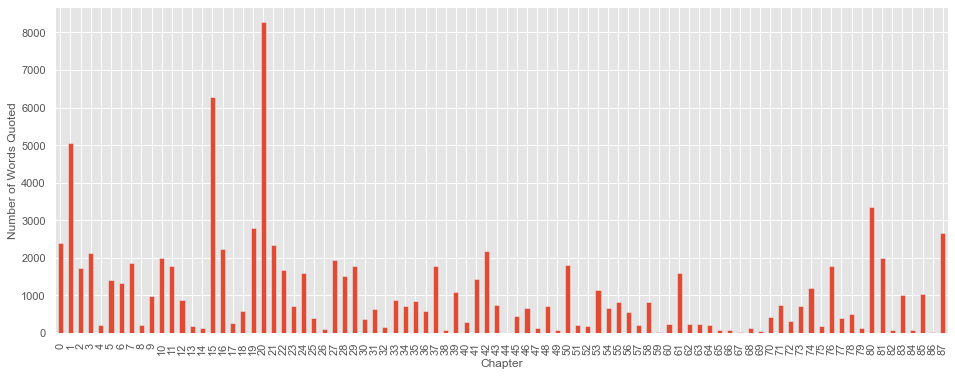
\includegraphics{byChapter.png}
\caption{Number of quotations of \emph{Middlemarch} by
chapter}\label{fig:byChapter}
}
\end{figure}

Next, we set out to discover the histories of these quotation patterns,
by grouping them by year of publication.
Fig.~\ref{fig:byChapterDiachronic} shows the same breakdown of
quotations per chapter, but shown across seven decades. What we found
surprised us---with the exception of Chapter 20, which has remained the
perennial favorite among scholars, other chapters have rises and falls
over 20- to 30--year cycles, becoming more quoted for a time, and then
gradually less quoted.\footnote{Given the precision and recall described
  above, our positive matches are highly reliable data, but we want to
  avoid making claims about the absence of matches. Nonetheless, our
  manual check of a subset of 56 items suggests that the data-matcher's
  false negatives weren't biased towards particular parts of the novel.}

\begin{figure}
\hypertarget{fig:byChapterDiachronic}{%
\centering
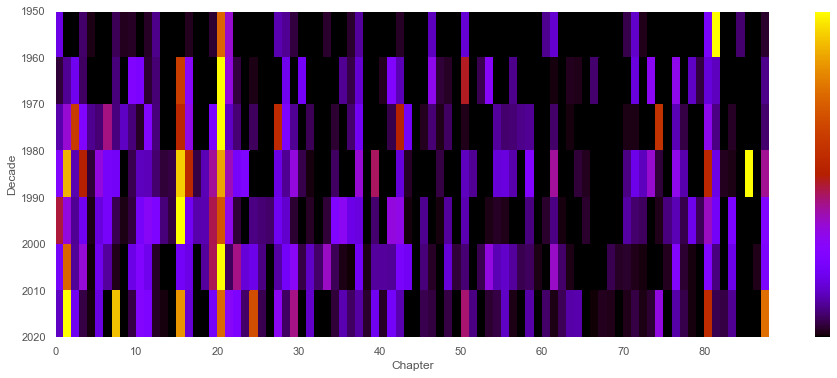
\includegraphics{byChapterDiachronic.png}
\caption{Number of quotations of \emph{Middlemarch} by chapter,
1950--2020}\label{fig:byChapterDiachronic}
}
\end{figure}

We discovered that Chapter 20 is the most-quoted chapter, due to large
numbers of quotations of its fifth and sixth paragraphs. This led us to
develop an even more granular visualization of quotation patterns: we
created
\href{https://lit-mod-viz.github.io/middlemarch-critical-histories/annotated.html}{a
text browser}, in which passages are colored according to the relative
number of quotations: darker-colored passages are less quoted, and
lighter-colored texts are more quoted. Fig.~\ref{fig:annotated} shows a
screenshot from this text browser, showing the most quoted passage in
the novel, from Chapter 20.

\begin{figure}
\hypertarget{fig:annotated}{%
\centering
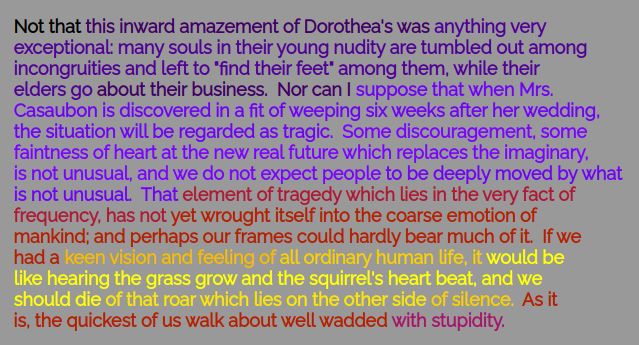
\includegraphics{annotated.png}
\caption{Annotated edition of \emph{Middlemarch}, by numbers of
quotations}\label{fig:annotated}
}
\end{figure}

Our inspiration for this browser comes from JSTOR's \emph{Understanding}
series. When we began our project, JSTOR had produced browsable texts of
Shakespeare plays and the US Constitution, annotated according to the
number of JSTOR text quoting from them. There are now many more texts
available for exploration, including \emph{Middlemarch}. But while
JSTOR's browser provides paragraph-level counts of quotations, our
analyses are accurate to the character level. This enabled us to find,
for example, that of this most-quoted sentence above, its beginning, `if
we had a,' is quoted much less than the rest of the sentence.

Our findings on the `squirrel's heart beat' passage led us to
investigate whether there were any patterns to quoted phrases. We thus
tallied all the words that appear in quotations, weighted them according
to numbers of quotations, and compared these word frequencies to the
words that didn't appear in our matches. The words most distinctive of
our quoted passages were, in order, \emph{life, like, woman, dorothea,
love, world, soul, consciousness, little, sort, deep, live, nature,} and
\emph{history}. Apart from the protagonist's name, Dorothea, the rest
are chiefly abstractions. This leads us to ask whether scholars are
drawn to quote passages that contain abstract claims---for example
claims about \emph{life, love,} or the \emph{soul}---because they
provide a more general purchase on a text than, say, a one-off plot
point or a detail from a description. Individual scholars may of course
quote plot points or descriptions, but collectively the shared reference
points are likely to be more abstract.\footnote{Stanford's Literary Lab
  has found similar patterns of quoted words within the British
  Periodicals Online corpus.}

We offer these results not as definitive of \emph{Middlemarch}, let
alone of scholarly quotation in general, but as an indication of the
kinds of research questions concerning textual history and disciplinary
practices that text-reuse detection can open onto. The results also show
the symbiosis between methods and findings: our adaptations to the
specificities of scholarly quotation gives us better results, whose
advantages and limitations we understand more precisely, and examining
the results prompts methodological refinements, as well as awareness of
quirks that may be particular to a given source text or scholarly
writer.

\hypertarget{conclusion}{%
\section{Conclusion}\label{conclusion}}

In this article, we've shown the importance of corpus-adapted studies of
text reuse, using our case study in literary scholarship of a single
source text (George Eliot's \emph{Middlemarch}) and a corpus of JSTOR's
scholarly writings. We've adapted our workflow to this corpus by tuning
hyperparameters like edit distance and number of n-grams matched on to
reflect the particular conventions of quotation post-1945 scholarship.
Our goal has been to provide a workflow for others to study quotations
from source texts in corpora of scholarly writings, and to provide a
clear pipeline for others using which is available for use on our GitHub
repository. While we continue to refine our matching algorithm, our goal
has been to illustrate some of the parameter tuning that comes with
detecting quotations within a humanities field where quotations compose
a significant portion of scholarly writings. Our case study has been in
literary studies, but we urge digital humanists of all disciplines to
make corpus-specific adaptations in their text-reuse detection studies.
Text-reuse detection isn't one-size-fits-all. More speculatively, our
workflow might be adapted to other corpora with other conventions: for
instance, instances of text from an early modern medical treatise like
Burton's \emph{Anatomy of Melancholy} quoted within eighteenth-century
scholarship (where differences in OCR quality and typographical
conventions like the long s might require a fuzzier edit distance). Or
we might imagine instances where a source text is highly repetitious,
where and additional level of tuning would be required to determine
which one of several instances in of phrase in a text is being quoted.
In the case of Middlemarch, there are few quotations that would be
repeated text. You would need to adapt to a specific corpus if the
source text is one where there is lots of repetition. Or we might
imagine instances in a smaller corpus, say, quotation from a piece of
legislation in a another legal text, where it might matter to identity
quotations smaller than five words, and where scholars might construct a
probability table examining the likelihood of a given n-gram in the
larger corpus. Without exhaustively listing the different kinds of
corpora or conventions, our hope is to provide a foundation and clear
workflow for adapting to more localized methods for studying text-reuse.

\hypertarget{acknowledgements}{%
\section{Acknowledgements}\label{acknowledgements}}

For their support on this project, we thank Dennis Yi Tenen, Alex Gil,
Roopika Risam, the Literary Modeling and Visualization Workshop at
Columbia University, and the contributors to the text-matcher open
source project.

\theendnotes

\hypertarget{references}{%
\section*{References}\label{references}}
\addcontentsline{toc}{section}{References}

\hypertarget{refs}{}
\begin{CSLReferences}{1}{0}
\leavevmode\vadjust pre{\hypertarget{ref-altschul1990basic}{}}%
\textbf{Altschul, S. F. et al.} (1990) Basic local alignment search
tool. \emph{Journal of molecular biology}. 215 (3), 403--410.

\leavevmode\vadjust pre{\hypertarget{ref-ArnoldLottev12022}{}}%
\textbf{Arnold, F.} (2022a) \emph{Lotte v1.3.0}. {Zenodo}.
\url{https://zenodo.org/record/6123229} (Accessed 19 May 2022).

\leavevmode\vadjust pre{\hypertarget{ref-ArnoldQuid2022}{}}%
\textbf{Arnold, F.} (2022b) \emph{Quid v.2.0.4}. {Zenodo}.
\url{https://zenodo.org/record/6525057} (Accessed 19 May 2022).

\leavevmode\vadjust pre{\hypertarget{ref-ArnoldLotteAnnetteFramework}{}}%
\textbf{Arnold, F. \& Jäschke, R.} (n.d.) \emph{Lotte and {Annette}: {A
Framework} for {Finding} and {Exploring Key Passages} in {Literary
Works}}.
\url{https://amor.cms.hu-berlin.de/~arnolfre/paper/NLP4DH_2021_arnold_lotte_preprint.pdf}.
\url{https://amor.cms.hu-berlin.de/~arnolfre/paper/NLP4DH_2021_arnold_lotte_preprint.pdf}.

\leavevmode\vadjust pre{\hypertarget{ref-AuyoungWhatWeMean2020}{}}%
\textbf{Auyoung, E.} (2020) What {We Mean} by {Reading}. \emph{New
Literary History}. 51 (1), 93--114.
\url{http://muse.jhu.edu/article/753316} (Accessed 11 August 2020).

\leavevmode\vadjust pre{\hypertarget{ref-BarTextReuseDetection2012}{}}%
\textbf{Bär, D. et al.} (2012) Text {Reuse Detection Using} a
{Composition} of {Text Similarity Measures}. \emph{Proceedings of COLING
2012}. 1167--184.
\url{https://www.cdc.informatik.tu-darmstadt.de/fileadmin/user_upload/Group_UKP/publikationen/2012/COLING_2012_DaB_published.pdf}
(Accessed 13 March 2016).

\leavevmode\vadjust pre{\hypertarget{ref-BuchlerMeasuringInfluenceWork2013}{}}%
\textbf{Büchler, M. et al.} (2013) Measuring the {Influence} of a {Work}
by {Text-Reuse}. \emph{Bulletin of the Institute of Classical Studies.
Supplement}. (122), 63--79. \url{https://www.jstor.org/stable/44216323}.

\leavevmode\vadjust pre{\hypertarget{ref-Budakdirectphonologydphon2021}{}}%
\textbf{Budak, N. et al.} (2021) \emph{Direct-phonology/dphon: 2.0.1}.
{Zenodo}. \url{https://zenodo.org/record/4641277} (Accessed 19 May
2022).

\leavevmode\vadjust pre{\hypertarget{ref-Budakdphon2022}{}}%
\textbf{Budak, N. \& Rominger, G. D.} (2022) \emph{Dphon}. {DIRECT}.
\url{https://github.com/direct-phonology/dphon} (Accessed 26 May 2022).

\leavevmode\vadjust pre{\hypertarget{ref-BuurmaEpigraphsMatter2012}{}}%
\textbf{Buurma, R. S.} (2012) Do {Epigraphs Matter}? The New Republic
\url{https://newrepublic.com/article/110640/art-epigraph-how-great-books-begin-rosemary-ahern}
(Accessed 19 May 2022).
\url{https://newrepublic.com/article/110640/art-epigraph-how-great-books-begin-rosemary-ahern}
(Accessed 19 May 2022).

\leavevmode\vadjust pre{\hypertarget{ref-CarpenterMEDICALCOSMOPOLITANISMMIDDLEMARCH2010}{}}%
\textbf{Carpenter, M. W.} (2010) {Medical Cosmopolitanism}:
"{Middlemarch}", {Cholera}, {and the Pathologies of English
Masculinity}. \emph{Victorian Literature and Culture}. 38 (2), 511--528.
\url{https://www.jstor.org/stable/25733489}.

\leavevmode\vadjust pre{\hypertarget{ref-CloughMETERMEasuringTExt2002}{}}%
\textbf{Clough, P. D. et al.} (2002) {METER}: {MEasuring TExt Reuse}.
\emph{Proceedings of the 40th Annual Meeting of the Association for
Computational Linguistics (ACL), Philadelphia}. 152--159.

\leavevmode\vadjust pre{\hypertarget{ref-CompagnonSecondeMainOu1979}{}}%
\textbf{Compagnon, A.} (1979) \emph{La {Seconde Main} : {Ou}, {Le
Travail} de la {Citation}}. {Paris}: {Seuil}.

\leavevmode\vadjust pre{\hypertarget{ref-DamesNotCloseReading2010a}{}}%
\textbf{Dames, N.} (2010) {`On {Not Close Reading}: {The Prolonged
Excerpt} as {Victorian Critical Protocol}'}, in Rachel Ablow (ed.)
\emph{The {Feeling} of {Reading}: {Affective Experience} \& {Victorian
Literature}}. {Ann Arbor}: {University of Michigan Press}. pp. 11--26.

\leavevmode\vadjust pre{\hypertarget{ref-donaldson1981}{}}%
\textbf{Donaldson, J. L. et al.} (1981) A plagiarism detection system.
\emph{SIGCSE Bull.} 13 (1), 21--25.
\url{https://doi.org/10.1145/953049.800955}.

\leavevmode\vadjust pre{\hypertarget{ref-DuhaimeTextualReuseEighteenth2016}{}}%
\textbf{Duhaime, D. E.} (2016) Textual {Reuse} in the {Eighteenth
Century}: {Mining Eliza Haywood}'s {Quotations}. \emph{Digital
Humanities Quarterly}. 010 (1),.

\leavevmode\vadjust pre{\hypertarget{ref-EarhartCitationalPoliticsQuantifying2021}{}}%
\textbf{Earhart, A. E. et al.} (2021) Citational politics: {Quantifying}
the influence of gender on citation in {Digital Scholarship} in the
{Humanities}. \emph{Digital Scholarship in the Humanities}. 36 (3),
581--594. \url{https://doi.org/10.1093/llc/fqaa011} (Accessed 19 May
2022).

\leavevmode\vadjust pre{\hypertarget{ref-FerberCitationsAreThey1986}{}}%
\textbf{Ferber, M. A.} (1986) Citations: {Are They} an {Objective
Measure} of {Scholarly Merit}? \emph{Signs: Journal of Women in Culture
and Society}. 11 (2), 381--389.
\url{https://www.journals.uchicago.edu/doi/10.1086/494230} (Accessed 19
May 2022).

\leavevmode\vadjust pre{\hypertarget{ref-GanasciaAutomaticdetectionreuses2014}{}}%
\textbf{Ganascia, J.-G. et al.} (2014) Automatic detection of reuses and
citations in literary texts. \emph{Literary and Linguistic Computing}.
29 (3), 412--421.
\url{https://academic.oup.com/dsh/article/29/3/412/986406/Automatic-detection-of-reuses-and-citations-in}
(Accessed 31 March 2017).

\leavevmode\vadjust pre{\hypertarget{ref-GarberQuotationMarks1999}{}}%
\textbf{Garber, M.} (1999) " " ({Quotation Marks}). \emph{Critical
Inquiry}. 25 (4), 653--679. \url{https://www.jstor.org/stable/1344098}.

\leavevmode\vadjust pre{\hypertarget{ref-GessnerBiblicalintertextualitydigital2013}{}}%
\textbf{Geßner, A. et al.} (2013) {`Biblical intertextuality in a
digital world: The tool {GERTRUDE}'}, in \emph{Proceedings of the 1st
{International Workshop} on {Collaborative Annotations} in {Shared
Environment}: Metadata, vocabularies and techniques in the {Digital
Humanities}}. {DH-CASE} '13. 10 September 2013 {New York, NY, USA}:
{Association for Computing Machinery}. pp. 1--5.
\url{https://doi.org/10.1145/2517978.2517985} (Accessed 18 May 2022).

\leavevmode\vadjust pre{\hypertarget{ref-HackReapingSomethingNew2016}{}}%
\textbf{Hack, D.} (2016) \emph{Reaping {Something New}: {African
American Transformations} of {Victorian Literature}}. {Princeton
University Press}. \url{https://books.google.com?id=iXCeDAEACAAJ}.

\leavevmode\vadjust pre{\hypertarget{ref-HumphreysHowJSTORLabs2017}{}}%
\textbf{Humphreys, A.} (2017) {`\emph{How {JSTOR Labs Applies} ({Some})
{Methods} \& {Tools} from {Digital Scholarship}}'}, in 30 October 2017
{Philadelphia}: Society for Scholarly Publishing.

\leavevmode\vadjust pre{\hypertarget{ref-KhritankovDiscoveringtextreuse2015}{}}%
\textbf{Khritankov, A. S. et al.} (2015) {`Discovering text reuse in
large collections of documents: {A} study of theses in history
sciences'}, in \emph{2015 {Artificial Intelligence} and {Natural
Language} and {Information Extraction}, {Social Media} and {Web Search
FRUCT Conference} ({AINL-ISMW FRUCT})}. November 2015 pp. 26--32.

\leavevmode\vadjust pre{\hypertarget{ref-KokkinakisDetectingReuseBiblical2016}{}}%
\textbf{Kokkinakis, D. \& Malm, M.} (2016) Detecting {Reuse} of
{Biblical Quotes} in {Swedish} 19th {Century Fiction} using {Sequence
Alignment}`. \emph{Corpus-based Research in the Humanities workshop
(CRH). December, 10. Warsaw, Poland.} 79--86.

\leavevmode\vadjust pre{\hypertarget{ref-KolakGeneratingLinksMining2008}{}}%
\textbf{Kolak, O. \& Schilit, B. N.} (2008) {`Generating {Links} by
{Mining Quotations}'}, in \emph{Proceedings of the {Nineteenth ACM
Conference} on {Hypertext} and {Hypermedia}}. {HT} '08. 2008 {New York,
NY, USA}: {ACM}. pp. 117--126.
\url{http://doi.acm.org/10.1145/1379092.1379117} (Accessed 27 March
2017).

\leavevmode\vadjust pre{\hypertarget{ref-KramnickCriticismTruth2020}{}}%
\textbf{Kramnick, J.} (2020) Criticism and {Truth}. \emph{Critical
Inquiry}. 47 (2), 218--240.
\url{http://www.journals.uchicago.edu/doi/10.1086/712118} (Accessed 15
January 2021).

\leavevmode\vadjust pre{\hypertarget{ref-levenshtein1966binary}{}}%
\textbf{Levenshtein, V. I. et al.} (1966) {`Binary codes capable of
correcting deletions, insertions, and reversals'}, in \emph{Soviet
physics doklady}. 1966 Soviet Union. pp. 707--710.

\leavevmode\vadjust pre{\hypertarget{ref-heng2010}{}}%
\textbf{Li, H. \& Homer, N.} (2010) {A survey of sequence alignment
algorithms for next-generation sequencing}. \emph{Briefings in
Bioinformatics}. 11 (5), 473--483.
\url{https://doi.org/10.1093/bib/bbq015}.

\leavevmode\vadjust pre{\hypertarget{ref-LinderTextPolicyMeasuring2020}{}}%
\textbf{Linder, F. et al.} (2020) Text as {Policy}: {Measuring Policy
Similarity} through {Bill Text Reuse}. \emph{Policy Studies Journal}. 48
(2), 546--574.
\url{http://onlinelibrary.wiley.com/doi/abs/10.1111/psj.12257} (Accessed
19 May 2022).

\leavevmode\vadjust pre{\hypertarget{ref-lukashenko2007}{}}%
\textbf{Lukashenko, R. et al.} (2007) {`Computer-based plagiarism
detection methods and tools: An overview'}, in \emph{Proceedings of the
2007 international conference on computer systems and technologies}.
CompSysTech '07. 2007 New York, NY, USA: Association for Computing
Machinery. \url{https://doi.org/10.1145/1330598.1330642}.

\leavevmode\vadjust pre{\hypertarget{ref-McMurtrieWhyPlagiarismDetectionCompany2019}{}}%
\textbf{McMurtrie, B.} (2019) \emph{Why a {Plagiarism-Detection Company
Is Now} a {Billion-Dollar Business}}
\url{http://www.chronicle.com/article/why-a-plagiarism-detection-company-is-now-a-billion-dollar-business/}
(Accessed 24 August 2022).

\leavevmode\vadjust pre{\hypertarget{ref-meckier1978arduous}{}}%
\textbf{Meckier, J.} (1978) "That arduous invention": Middlemarch versus
the modern satirical novel. \emph{ARIEL: A Review of International
English Literature}. 9 (4),.

\leavevmode\vadjust pre{\hypertarget{ref-MeyerPoeticsQuotationEuropean2015}{}}%
\textbf{Meyer, H.} (2015) \emph{The {Poetics} of {Quotation} in the
{European Novel}}. {Princeton University Press}.
\url{https://books.google.com?id=whjWCgAAQBAJ}.

\leavevmode\vadjust pre{\hypertarget{ref-MillerQuoteNotQuote}{}}%
\textbf{Miller, D.} (n.d.) \emph{To {Quote} or {Not} to {Quote}}
\url{http://shakespeare.visualizingbroadway.com/index.html} (Accessed 19
May 2022).

\leavevmode\vadjust pre{\hypertarget{ref-MilletUnionMissBrooke1980}{}}%
\textbf{Millet, S.} (1980) The {Union} of "{Miss Brooke}" and
"{Middlemarch}": {A Study} of the {Manuscript}. \emph{The Journal of
English and Germanic Philology}. 79 (1), 32--57.
\url{https://www.jstor.org/stable/27708593}.

\leavevmode\vadjust pre{\hypertarget{ref-MoleWhatVictoriansMade2017}{}}%
\textbf{Mole, T.} (2017) \emph{What the {Victorians Made} of
romanticism: Material artifacts, cultural practices, and reception
history}. {Princeton}: {Princeton University Press}.

\leavevmode\vadjust pre{\hypertarget{ref-LincolnAmericaPublicBible}{}}%
\textbf{Mullen, L.} (2016) \emph{America's {Public Bible}: {Biblical
Quotations} in {U}.{S}. {Newspapers}}
\url{https://americaspublicbible.org/} (Accessed 13 May 2022).

\leavevmode\vadjust pre{\hypertarget{ref-QuotationFinderAmerica2022}{}}%
\textbf{Mullen, L.} (2022) \emph{Quotation {Finder} \textbar{}
{America}'s {Public Bible}}. {America's Public Bible}.
\url{https://github.com/public-bible/quotation-finder} (Accessed 13 May
2022).

\leavevmode\vadjust pre{\hypertarget{ref-NichollsDetectingTextualReuse2019}{}}%
\textbf{Nicholls, T.} (2019) Detecting {Textual Reuse} in {News
Stories}, {At Scale}. \emph{International Journal of Communication}. 13
(0, 0), 25. \url{https://ijoc.org/index.php/ijoc/article/view/9904}
(Accessed 13 May 2022).

\leavevmode\vadjust pre{\hypertarget{ref-OlsenSomethingBorrowedSequence2011}{}}%
\textbf{Olsen, M. et al.} (2011) Something {Borrowed}: {Sequence
Alignment} and the {Identification} of {Similar Passages} in {Large Text
Collections}. \emph{Digital Studies / Le champ numérique}. 2 (1, 1),.
\url{https://www.digitalstudies.org/article/id/7224/} (Accessed 19 May
2022).

\leavevmode\vadjust pre{\hypertarget{ref-paice1990}{}}%
\textbf{Paice, C. D.} (1990) Another stemmer. \emph{SIGIR Forum}. 24
(3), 56--61. \url{https://doi.org/10.1145/101306.101310}.

\leavevmode\vadjust pre{\hypertarget{ref-peters_difflib_2016}{}}%
\textbf{Peters, T.} (2016) \emph{Difflib}. {Python Software Foundation}.
\url{https://docs.python.org/3.5/_sources/library/difflib.txt} (Accessed
19 March 2016).

\leavevmode\vadjust pre{\hypertarget{ref-PiperMeasuringUnreading2020}{}}%
\textbf{Piper, A. \& Manalad, J.} (2020) Measuring {Unreading}.
\emph{Goethe Yearbook}. 27 (1), 233--241.
\url{https://muse.jhu.edu/article/762250} (Accessed 9 September 2020).

\leavevmode\vadjust pre{\hypertarget{ref-PriceAnthologyRiseNovel2000}{}}%
\textbf{Price, L.} (2000) \emph{The {Anthology} and the {Rise} of the
{Novel}}. {Cambridge, UK}: {Cambridge University Press}.

\leavevmode\vadjust pre{\hypertarget{ref-PrinsVictorianSappho1999}{}}%
\textbf{Prins, Y.} (1999) \emph{Victorian {Sappho}}. {Princeton, N.J}:
{Princeton University Press}.

\leavevmode\vadjust pre{\hypertarget{ref-ratcliff1988pattern}{}}%
\textbf{Ratcliff, J. W. \& Metzener, D. E.} (1988) Pattern-matching-the
gestalt approach. \emph{Dr Dobbs Journal}. 13 (7), 46.

\leavevmode\vadjust pre{\hypertarget{ref-RoeDiggingECCOIdentifying2016}{}}%
\textbf{Roe, G. et al.} (2016) Digging into {ECCO}: {Identifying
Commonplaces} and other {Forms} of {Text Reuse} at {Scale}.
\emph{Digital Humanities 2016: Conference Abstracts. Jagiellonian
University \& Pedagogical University, Kraków}. 336--339.

\leavevmode\vadjust pre{\hypertarget{ref-RomanelloExploringCitationNetworks2016}{}}%
\textbf{Romanello, M.} (2016) Exploring {Citation Networks} to {Study
Intertextuality} in {Classics}. \emph{Digital Humanities Quarterly}. 010
(2),.

\leavevmode\vadjust pre{\hypertarget{ref-SeoLocaltextreuse2008}{}}%
\textbf{Seo, J. \& Croft, W. B.} (2008) {`Local text reuse detection'},
in \emph{Proceedings of the 31st annual international {ACM SIGIR}
conference on {Research} and development in information retrieval}.
{SIGIR} '08. 20 July 2008 {New York, NY, USA}: {Association for
Computing Machinery}. pp. 571--578.
\url{https://doi.org/10.1145/1390334.1390432} (Accessed 13 May 2022).

\leavevmode\vadjust pre{\hypertarget{ref-CiteBlackWomenCollectiveCiteBlackWomen}{}}%
\textbf{Smith, C. A.} (2017) \emph{Cite {Black Women}.}
\url{https://www.citeblackwomencollective.org/} (Accessed 30 January
2021).

\leavevmode\vadjust pre{\hypertarget{ref-SmithDetectingModelingLocal2014}{}}%
\textbf{Smith, D. A. et al.} (2014) {`Detecting and {Modeling Local Text
Reuse}'}, in \emph{Proceedings of the 14th {ACM}/{IEEE-CS Joint
Conference} on {Digital Libraries}}. {JCDL} '14. 2014 {Piscataway, NJ,
USA}: {IEEE Press}. pp. 183--192.
\url{http://dl.acm.org/citation.cfm?id=2740769.2740800} (Accessed 31
March 2017).

\leavevmode\vadjust pre{\hypertarget{ref-SmithInfectioustextsModeling2013}{}}%
\textbf{Smith, D. A. et al.} (2013) {`Infectious texts: {Modeling} text
reuse in nineteenth-century newspapers'}, in \emph{2013 {IEEE
International Conference} on {Big Data}}. October 2013 pp. 86--94.

\leavevmode\vadjust pre{\hypertarget{ref-SturgeonUnsupervisedidentificationtext2018}{}}%
\textbf{Sturgeon, D.} (2018) Unsupervised identification of text reuse
in early {Chinese} literature. \emph{Digital Scholarship in the
Humanities}. 33 (3), 670--684. \url{https://doi.org/10.1093/llc/fqx024}
(Accessed 13 May 2022).

\leavevmode\vadjust pre{\hypertarget{ref-nltkLancaster}{}}%
\textbf{Tomcavage, S.} (2022) \emph{NLTK: Lancaster stemmer}. NLTK.
\url{https://www.nltk.org/_modules/nltk/stem/lancaster.html} (Accessed
26 May 2022).

\leavevmode\vadjust pre{\hypertarget{ref-VesantoSystemIdentifyingExploring2017}{}}%
\textbf{Vesanto, A., Ginter, F., et al.} (2017) {`A {System} for
{Identifying} and {Exploring Text Repetition} in {Large Historical
Document Corpora}'}, in \emph{Proceedings of the 21st {Nordic
Conference} on {Computational Linguistics}}. May 2017 {Gothenburg,
Sweden}: {Association for Computational Linguistics}. pp. 330--333.
\url{https://aclanthology.org/W17-0249} (Accessed 19 May 2022).

\leavevmode\vadjust pre{\hypertarget{ref-VesantoApplyingBLASTText2017}{}}%
\textbf{Vesanto, A., Nivala, A., et al.} (2017) \emph{Applying {BLAST}
to {Text Reuse Detection} in {Finnish Newspapers} and {Journals},
1771--1910}. 5.

\end{CSLReferences}

\end{document}
